% ---------------------------------------------------------------------
% HEADER
% Formålet med å legge header til et eget dokument er å garantere at
% oppsettet av dokumentene er likt for alle løsningsforslagene.
% I headeren skjer følgende:
% (1) Dokumentet blir startet
% (2) Pakker blir importert
% ---------------------------------------------------------------------
% ---------------------------------------------------------------------
% HEADER
% Formålet med header er å importere de samme pakkene i alle dokumentene.
% ---------------------------------------------------------------------

% Sett opp dokumentet. Her kan 'twoside' brukes for printing
\documentclass[12pt, a4paper]{article}

% Vi trenger utf-8 for å bruke norske bokstaver: Æ, Ø, Å
\usepackage[utf8]{inputenc}

% Vi setter babel til norsk, da får dokumentegenskaper norske titler
\usepackage[norsk]{babel}

% For å kunne bruke grafikk
\usepackage{graphicx}
\newcommand{\figwidth}{0.75}

% Matematikkpakker fra AMS - American Mathematical Society
\usepackage{amsmath, amsthm, amsfonts, amssymb, mathtools}

% For eventuelle linker, e.g. \href{URL}{text}
\usepackage{hyperref}

% For headers og footers med eventuell logo
\usepackage{fancyhdr}

% Sett marginer manuelt
\usepackage[top = 3cm, left = 3cm, right = 3cm, bottom = 3cm]{geometry}

% For enkle lister, nyttig for oppgave a), b), c), ...
\usepackage[sharp]{easylist}

% Dersom flere kolonner er ønskelig i deler av dokumentet
\usepackage{multicol}

% For luft mellom paragrafer
\usepackage{parskip}

% For logikk assosiert med logoer
\usepackage{ifthen}

% For å finne totalt antall sider
\usepackage{lastpage}

% Annet
\usepackage{enumitem}

\usepackage{polynom}% Polynomer
\polyset{style=C, div=:}

\usepackage{systeme}% Likningssystemer

% Kan brukes når noe stryker ut noe, f.eks 1/n * n, her kan man ta \frac{1}{\cancel{n}} * \cancel{n}
\usepackage{cancel}



% ---------------------------------------------------------------------
% DOKUMENTVARIABLER
% ---------------------------------------------------------------------
\newcommand{\fagkode}{S2}
\newcommand{\semesteraar}{våren 2014}
\newcommand{\forfatter}{Tommy O.}
\newcommand{\dokumenttittel}{Løsningsforslag -- Eksamen \fagkode, \semesteraar}


% Set til 'true' og oppgi logo dersom du vil bruke en logo
\newboolean{bruklogo}
\setboolean{bruklogo}{true}
\newcommand{\logonavn}{figs/metis_akademiet_privatistskole_doclogo.png}

% ---------------------------------------------------------------------
% SETUP
% Formålet med å legge setup til et eget dokument å garantere at headers,
% footers, og øverste del av dokumentet er likt for alle
% løsningsforslagene.
% ---------------------------------------------------------------------
% ---------------------------------------------------------------------
% HEADER
% Formålet med setup er at dokumentene ser rimelig like ut.
% ---------------------------------------------------------------------


% ---------------------------------------------------------------------
% Alternativ font. Kommentert ut fordi Computer Modern (default) er pen
%\usepackage{kmath,kerkis}
%\usepackage[T1]{fontenc}
% ---------------------------------------------------------------------


% ---------------------------------------------------------------------
% Sett opp headers og footers
\ifthenelse{\boolean{bruklogo}}{
% Dersom logo skal brukes, sett logoen oppe til høyre med bredde 4 cm
	\rhead{\includegraphics[width=3.5cm]{\logonavn}}
}{
% Dersom logo ikke skal brukes, sett tom header
	\rhead{}
} 
\rfoot{\thepage}
\cfoot{}
\lhead{}
\lfoot{{\scriptsize Forbedringsforslag? Bidra på \url{https://github.com/tommyod/matte_eksamener_VGS}.}}
\renewcommand{\headrulewidth}{0pt}
% ---------------------------------------------------------------------


% ---------------------------------------------------------------------
% To streker under svaret
\def\answer#1{\underline{\underline{#1}}}
% ---------------------------------------------------------------------


% ---------------------------------------------------------------------
% Start selve dokumentet
% ---------------------------------------------------------------------

\begin{document}
\pagestyle{fancy}
{\bfseries \Large \dokumenttittel} \\
{ \footnotesize Laget av \forfatter 
	\hfill Sist oppdatert: \today 
	\hfill Antall sider: \pageref*{LastPage}}
\hrule
\vspace{1em}
\begin{center}
\fbox{\fbox{\parbox{.90\textwidth}{
	Dette dokumentet er open-source;
	alle kan bidra til å gjøre det bedre.
	Dersom du finner skrivefeil, matematiske feil, eller ser at forklaringene kan være bedre: ikke nøl med å sende inn en endring. 
	Du kan finne siste versjon, og bidra, på GitHub, se:
	\url{https://github.com/tommyod/matte_eksamener_VGS}
}}}
\end{center}


% ---------------------------------------------------------------------
% DOKUMENTSTART - Skriv løsningsforslaget nedenfor
% ---------------------------------------------------------------------	
\section*{Del 1 - uten hjelpemidler}
\subsection*{Oppgave 1}
\begin{easylist}[enumerate]
\ListProperties(Style2*=,Numbers=a,Numbers1=l,FinalMark={)})
# Vi skal derivere $f(x) = 3/x^2$. 
Vi skriver om til $f(x) = 3x^{-2}$ og deriverer slik
\begin{align*}
	f'(x) &= 3 \left(x^{-2}\right)' \\
	      & = 3 (-2)x^{-3} \\
	      & = \answer{-\frac{6}{x^3}}.
\end{align*}


# Vi skal derivere $g(x) = xe^{-4x}$, og må her bruke produkregelen
$(uv)' = u'v + uv'$ slik
\begin{align*}
	g'(x) &= \left(x \right)' e^{-4x} +x \left( e^{-4x} \right)' \\
	& = 1 e^{-4x} + x (-4) e^{-4x}  \\
	& = e^{-4x} -4x e^{-4x}  \\
	& =  \answer{e^{-4x} \left( 1 - 4x\right) }.
\end{align*}
\end{easylist}

\subsection*{Oppgave 2}
Vi ser på funksjonen
\begin{equation*}
	P(x) = x^3 - 3x^2 + 4, \qquad D_{P} = \mathbb{R}
\end{equation*}
\begin{easylist}[enumerate]
\ListProperties(Style2*=,Numbers=a,Numbers1=l,FinalMark={)})
# Vi setter inn $x=2$ i $P(x)$ og får $P(2) = (2)^3 - 3(2)^2 + 4 = 8 - 12 + 4 = \answer{0}$.
# Ettersom $P(2) = 0$, vet vi at $(x-2)$ må være en faktor i $P(x)$.
Vi utfører divisjonen og får \\
\polylongdiv{x^3 - 3x^2 + 4}{x - 2} \\
Nå vet vi at $P(x) = (x-2)(x^2 - x - 2)$, og ved hjelp av 
ABC formelen finner vi ut at $(x^2 - x - 2) = (x-2)(x+1)$,
altså kan vi faktorisere $P(x)$ som
\begin{equation*}
	\answer{P(x) = (x-2)^2 (x+1)}.
\end{equation*}
En enkel metode for å sjekke om dette svaret er riktig er å gange sammen disse faktorene og se at du får $P(x) = x^3 - 3x^2 + 4$ tilbake.

\end{easylist}


\subsection*{Oppgave 3}
\begin{easylist}[enumerate]
	\ListProperties(Style2*=,Numbers=a,Numbers1=l,FinalMark={)})
	# Dette er en aritmetisk rekke med $a_1 = 3$, differanse $d=3$
	og siste ledd $a_n = 300$. For å finne ut antall ledd $n$ kan
	vi bruke formelen $a_n = a_1 + d(n-1)$, vi får da
	\begin{align}
		\label{eqn:ledd_formel}a_n &= a_1 + d(n-1) \\
		\nonumber 300 &= 3 + 3(n-1) \\
		\nonumber 99 &= n-1 \\
		\nonumber n &= 100. 
	\end{align}
	Nå har vi alt vi trenger for å bruke summeformelen for en artimetisk
	rekke, vi løser slik
	\begin{equation*}
		S = \left(\frac{a_1 + a_n}{2}\right)n 
		= \left(\frac{3 + 300}{2}\right)100
		= 303(50) = \frac{30300}{2} = \answer{15150}.
	\end{equation*}
	# Dersom $a_1 = 4$ kan vi bruke formelen og finne ut at $a_3 = a_1 + 8 = 4 + 8 = 12$.
	Vi setter så dette inn i formel \eqref{eqn:ledd_formel} brukt i forrige oppgave, og får at 
	\begin{equation*}
		a_3 = a_1 + d(3 -1) \quad \Leftrightarrow 
		\quad 12 = 4 + d 2  \quad \Leftrightarrow 
		\quad d = 4,
	\end{equation*}
	og da må $a_2 = a_1 + d = 4 + 4 = \answer{8}$.
\end{easylist}



\subsection*{Oppgave 4}
Vi bruker følgende variabler: $v$ er antall voksne, $b$ er antall barn og $p$ er antall pensjonister som møtte på konserten.
Hver setning gir oss én likning:
\begin{easylist}[itemize]
	%\ListProperties(Style2*=,Numbers=a,Numbers1=l,FinalMark={)})
	# ``Det ble solgt 80 billetter.'' $\quad \Rightarrow \quad v + b + p = 80 \quad \text{(A)}$
	# ``Billettinntektene var 5000 kroner.'' 
	$\quad \Rightarrow \quad 100v + 50b + 60p = 5000 \quad \text{(B)}$
	# ``Like mange til barn som til voksne og pensjonister til sammen.'' \\ $\quad \Rightarrow \quad - v + b - p = 0 \quad \text{(C)}$
\end{easylist}
Vi legger sammen likning $(A)$ og likning $(C)$, og får at $2b = 80$,
altså er $\answer{b=40}$.
Deretter setter vi $b = 40$ inn i likning $(A)$ og $(B)$, og får
\begin{align*}
	v + p &= 40 \quad \text{(D)}\\
	100v  + 60p &= 3000\quad \text{(E)}
\end{align*}
Vi regner ut $100 \times \text{(D)} - \text{(E)}$, og får at $40p = 1000$.
Da er $\answer{p = 25}$, setter vi inn dette i likning $\text{(D)}$ finner vi også ut at $\answer{v = 15}$.



\subsection*{Oppgave 5}
\begin{easylist}[enumerate]
\ListProperties(Style2*=,Numbers=a,Numbers1=l,FinalMark={)})
# Generelt så har $f'(x)$ topp- og bunnpunkt når $f'(x) = 0$.
Her er $f'(x) = 0$ når $x = -2$ og når $x = 6$. 
Vi ser at \answer{$x=-2$ er et toppunkt} og \answer{$x=6$ er et bunnpunkt}. Grafen vokser når $f'(x) > 0$, og minker når $f'(x) < 0$. Vi ser også at \\ \answer{funksjonen vokser når $x < -2$ og når $x > 6$}, og \answer{minker når $ -2 < x < 6$}.
# Likningen for tangenten til $f(x)$ i et punkt $x_0$ er gitt ved
\begin{equation*}
	y = f(x_0) + f'(x_0) ( x - x_0).
\end{equation*}
Vi får oppgitt punktet $(x_0, f(x_0)) = (4, 3)$, og fra grafen til $f'(x)$
ser vi at $f'(x_0) = f'(4) = -3$. Vi får altså følgende tangentlinje:
\begin{align*}
	y &= f(x_0) + f'(x_0) ( x - x_0) \\
	y &= f(4) + f'(4) ( x - 4) \\
	y &= 3 + -3 ( x - 4) \\
	& \answer{y = -3x + 15 }
\end{align*}
# Funksjonen $f''(x)$ er positiv når $f'(x)$ stiger, og negativ når $f'(x)$ synker.
Med andre ord er $f''(x) < 0$ når $x < 2$, og $f''(x) > 0$ når $x > 2$.
Vendepunktet oppstår når $f''(x)$ endrer fortegn, altså når $\answer{x=2}$.

# Basert på den deriverte, samt kjennskap til bunnpunkt og toppunkt, burde du klare å lage en skisse som ligner på $f'(x)$ vist i Figur \ref{fig:del1_oppg5}.

\begin{figure}[ht!]
	\centering
	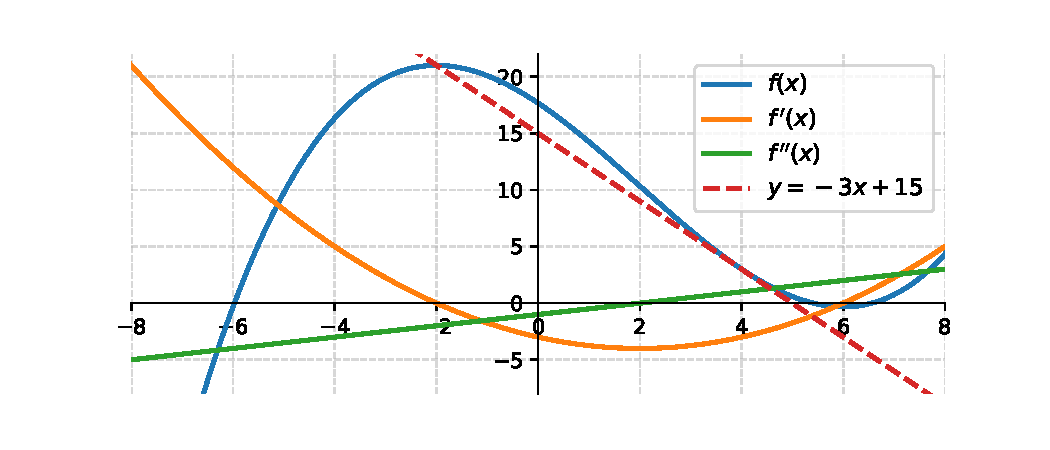
\includegraphics[width=0.85\linewidth]{figs/del1_oppg5}
	\caption{Funksjonene fra oppgave 5, del 1.}
	\label{fig:del1_oppg5}
\end{figure}
\end{easylist}

\subsection*{Oppgave 6}
\begin{easylist}[enumerate]
\ListProperties(Style2*=,Numbers=a,Numbers1=l,FinalMark={)})
# Her må vi bruke forventningsverdier og utfallsrom. Både $X_2$ og $X_4$ har $n > 10$, så disse må samsvare med figurene $(1)$ og $(3)$, ettersom disse har positive sannsynligheter for $X > 10$.
Ettersom $\operatorname{E}(X_2) = np = 100(0.06) = 6$ og $\operatorname{E}(X_4) = 5$, så velger vi $\answer{X_2 = (3)}$ og $\answer{X_4 = (1)}$,
ettersom dette samsvarer best med høyeste stolpe på figurene.
Basert på forventningsverdiene til $X_1$ og $X_3$ så velger vi $\answer{X_1 = (2)}$ og $\answer{X_3 = (4)}$.
# Det må være $\answer{X_2}$ (figur $(3)$), fordi alle andre arealer er for små.
Ettersom det er satt tall på aksene er det mulig å gjøre en grov utregning av arealet ved å lese av søylene, og da ser man at de andre er for små.
# Variabelen med størst standardavvik er den som har størst varians, ettersom
$\operatorname{SD}(X) = \sqrt{\operatorname{Var}(X)}$, og $a > b$ impliserer at $\sqrt{a} > \sqrt{b}$.
Når $X$ er binomisk fordelt er $\operatorname{Var}(X) = np(1-p)$, vi regner ut alle variansene (det er Del 1, så vi trenger ikke å regne nøye):
\begin{align*}
\operatorname{Var}(X_1) &= np(1-p) = 10 (0.6) 0.4 = 2.4 \\ 
\operatorname{Var}(X_2) &= np(1-p) = 100 (0.06) 0.94 \approx 6 \\
\operatorname{Var}(X_3) &= np(1-p) = 10 (0.4) 0.6 = 2.4 \\
\operatorname{Var}(X_4) &= np(1-p) = 50 (0.1) 0.9 = 4.5
\end{align*}
Vi ser at  \answer{$X_2$} har størst varians, og derfor også størst standardavvik.
\end{easylist}




\section*{Del 2 - med hjelpemidler}

\subsection*{Oppgave 1}
\begin{easylist}[enumerate]
\ListProperties(Style2*=,Numbers=a,Numbers1=l,FinalMark={)})
# Omkretsen til en sirkel er $O = 2 \pi r$, så halve omkretsen bli $\pi r$.
Vi ser at 
\begin{align*}
	O_1 &=  \frac{(2r)}{2} \pi = r \pi \\
	O_2 &=  \frac{(r)}{2} \pi = r \pi /2 \\
	O_3 &=  \frac{(r/2)}{2} \pi = r \pi / 2^2 \\
	\vdots &= \vdots \\
	O_n &=  \frac{(r/2^{n-2})}{2} \pi = r \pi / 2^{n-1},
\end{align*}
og summer blir en uendelig geometrisk rekke fordi
\begin{equation}
\label{eqn:geometrisk}
	S = O_1 + O_2  + \dots =  r \pi \left( 1 + \frac{1}{2} + 
	\frac{1}{2^2} + \frac{1}{2^3} + \dots \right)
\end{equation}
# Vi vet at $1 + k + k^2 + k^3 + \dots = 1/ (1-k)$, dette er summeformelen for en uendelig geometrisk rekke, og den konvergerer (går ikke mot evig) når $-1 < k < 1$. I denne oppgaven er $k = 1/2$, vi setter formelen inn i likning \eqref{eqn:geometrisk} og får 
\begin{equation*}
S =  r \pi \left( 1 + \frac{1}{2} + 
\frac{1}{2^2} + \frac{1}{2^3} + \dots \right)
=  r \pi \left( \frac{1}{1 - \frac{1}{2}} \right)
=  r \pi \left( \frac{1}{\frac{1}{2}} \right)
 = \answer{2 \pi r}.
\end{equation*}
I Geogebra kan du skrive \verb|S := r * (pi) * Sum(1/2^i, i, 0, |$\infty$\verb|)|.
\end{easylist}

\subsection*{Oppgave 2}

\begin{center}
	\begin{tabular}{|l|c|c|c|c|c|}
		\hline
		\textbf{Årstall} & 1990 & 1995 & 2000 & 2005 & 2010 \\ \hline
		\textbf{Antall døde jerv} & 2 & 16 & 41 & 63 & 105 \\ \hline
	\end{tabular}
\end{center}


\begin{easylist}[enumerate]
\ListProperties(Style2*=,Numbers=a,Numbers1=l,FinalMark={)})
# Her virker en lineær modell best, basert på hvordan linjen passer til datene, se Figur \ref{fig:del2_oppg2}.
# Evaluer funksjonen $y(x) = 5.06x - 5.2$ i punktet
$x = 24$. Vi får $y(24) = 5.06(24) - 5.2 = 116.24$.
Ifølge modellen kan vi forvente \answer{116} døde jerv registrert i 2014.

\begin{figure}[ht!]
	\centering
	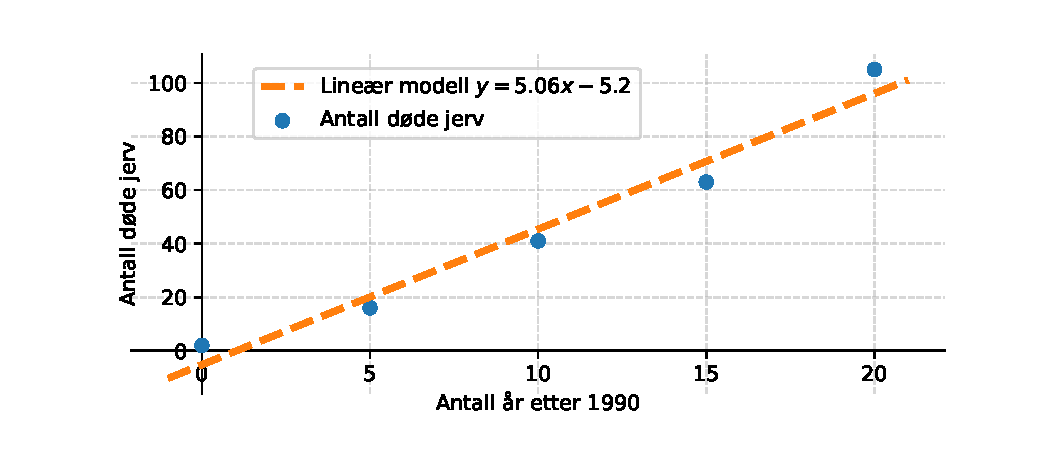
\includegraphics[width=0.85\linewidth]{figs/del2_oppg2}
	\caption{}
	\label{fig:del2_oppg2}
\end{figure}


# Vi kan løse på 2 forskjellige måter
## \verb|f(x) := 5.06*x - 5.2| \verb|Sum(f(x), x, 0, 24)| gir 1388
\end{easylist}


\subsection*{Oppgave 3}
\begin{easylist}[enumerate]
	\ListProperties(Style2*=,Numbers=a,Numbers1=l,FinalMark={)})
	# Vi legger dataene inn i regnearket i Geogebra, og velger en lineære regresjonsmodell. Vi får $p(x) = -0.224x +2219.17$.
	Inntekten er prisen ganget med antall varger solgt, vi får
	\begin{equation*}
		\answer{I(x) = p(x) \times x = -0.224x^2 +2219.17x}.
	\end{equation*}
	# Definer $I(x)$ og $K(x)$ i CAS ved å skrive inn \\
	\verb|I(x) := -0.22421189 * x^2 + 2219.1684 * x| (se notat\footnote{Her er det viktig å ta med rikelig med desimaler. Tar du med for få desimaler vil svarene i de neste oppgavene ikke bli like nøyaktige.})
	og  \\
	\verb|K(x) := 0.03 * x^2 + 15 * x + 605000|.
	Bruker deretter CAS til å regne ut:
	\begin{align*}
		I'(3000) &= 873.9\\
		K'(3000) &= 195\\
	\end{align*}
	Ettersom overskuddet $O(x) = I(x)  - K(x)$, vil overskuddet øke
	dersom $I'(x) > K'(x)$ og vi produserer mer.
	\answer{Vi bør øke produksjonen}.
	# Skriv inn \verb|Løs[I'(x) > K'(x), x]| i CAS, svaret blir
	\answer {$x < 4335.3$}.
	Vi bør produsere mer dersom vi produserer mindre enn 4335 varer.
	# Overskuddet $O(x)$ er størst når $O'(x) = 0$.
	Da er $I'(x) = K'(x)$, så vi skriver \verb|Løs[I'(x) = K'(x), x]|
	og får $x = 4335.3$ som svar. Bedriften må produsere og selge
	\answer{4335 enheter} for at overskuddet skal være størst\footnote{Det er ingen garanti for at å runde av $4335.3$ til $4335$ gir beste overskudd. Du kan sammenligne $O(4334)$, $O(4335)$ og $O(4336)$ og velge den største for å være sikker på at du har rett svar.}.
\end{easylist}

\subsection*{Oppgave 4}
\begin{easylist}[enumerate]
	\ListProperties(Style2*=,Numbers=a,Numbers1=l,FinalMark={)})
	# Vi bruker formelen for volum, og løser for $h$ slik:
	\begin{align*}
		\text{Volum} &= (\text{Høyde}) \times (\text{Bredde}) \times (\text{Lengde}) \\
		10 &= h  \times x \times 2x \\
		h &= \frac{5}{x^2}
	\end{align*}
	# Den totale kostnaden er summen av kostnad per kvadratmeter, ganget med areal i kvadratmeter, for alle sidene. Her er en detaljert forklaring.
	\begin{align*}
		\text{Total kostnad} &=  
		\underbrace{\frac{\text{Kostnad}}{m^2} \times m^2}_{\text{Sider}} + 
		\underbrace{\frac{\text{Kostnad}}{m^2} \times m^2}_{\text{Bunn}}
		\\
		\text{Total kostnad} &=  
		\underbrace{60 \times \left( 2(2x \times h + x \times h) \right)}_{\text{Sider}} + 
		\underbrace{100 \times \left( 2x \times x \right)}_{\text{Bunn}}
		\\
		K(x) &=  
		\underbrace{60 \times \left( 2\left(2x \times \frac{5}{x^2} + x \times \frac{5}{x^2}\right) \right)}_{\text{Sider}} + 
		\underbrace{100 \times \left( 2x \times x \right)}_{\text{Bunn}}
		\\
		K(x) &=  
		120 \times \left(  \frac{10}{x} +\frac{5}{x} \right) + 
		200x^2
		\\
		K(x) &=  \frac{1800}{x} + 
		200x^2
	\end{align*}
	
	# Definer funksjon med \verb|K(x) := 200x^2 + 1800/x| i CAS i Geogebra.
	Bruk deretter \verb|Ekstremalpunkt(K, 0.1, 10)| til å finne den minimale prisen. 
	Vi finner at $\answer{x = \text{bredde} = 1.64 \text{m}}$, 
	$\answer{2x = \text{lengde} = 3.3 \text{m}}$ og
	 $\answer{h = 5/x^2 = \text{høyde} = 1.83 \text{m}}$.
	 Den minste kostnaden ved å produsere containeren er
	 \answer{1635 kr}. Se Figur \ref{fig:del2_oppg4} for et skjembilde
	 av CAS-utregning.
	
\begin{figure}[ht!]
\centering
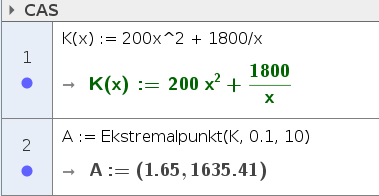
\includegraphics[width=0.5\linewidth]{figs/del2_oppg4}
\caption{Skjembilde av CAS for oppgave 4, del 2.}
\label{fig:del2_oppg4}
\end{figure}
\end{easylist}


\subsection*{Oppgave 5}
\begin{easylist}[enumerate]
	\ListProperties(Style2*=,Numbers=a,Numbers1=l,FinalMark={)})
	# La $X$ være antallet som blir trukket ut av $n = 3$ personer.
	Da er $X$ binomisk fordelt med $n=3$ og $p = 0.1$, og $P(X = 3)$ er gitt ved
	\begin{equation*}
		P(X = x) = \binom{n}{x} p^x (1-p)^{n-p} = 
		\binom{3}{3} 0.1^3 (1-0.1)^{3 -3} = 0.1^3 = \answer{0.001 = 0.1 \%}.
	\end{equation*}
	Det er enda enklere å tenke at tre personer må trekkes på rad, og at sannsynligheten for at én blir trukket er $p = 0.1$, så da er sannsynligheten for at tre blir trukket på rad lik $p^3 = 0.1^3 = 0.001 = 0.1 \%$.
	# Den stokastiske variabelen $X$ er binomisk fordelt med $n=1000$ og $p = 0.1$. Vi bruker formlene for forventning og standardavvik for binomisk fordeling.
	\begin{align*}
		\operatorname{E}(X) &= np = 1000 (0.1) = \answer{100}\\
		\operatorname{SD}(X) &= \sqrt{\operatorname{Var}(X)} 
		= \sqrt{np(1-p)} = \sqrt{1000 (0.1) (0.9)} = \answer{\sqrt{90} \approx 9.49}
	\end{align*}
	Fordelingen til $X$ er vist i Figur \ref{fig:del2_oppg5}.
	
\begin{figure}[ht!]
\centering
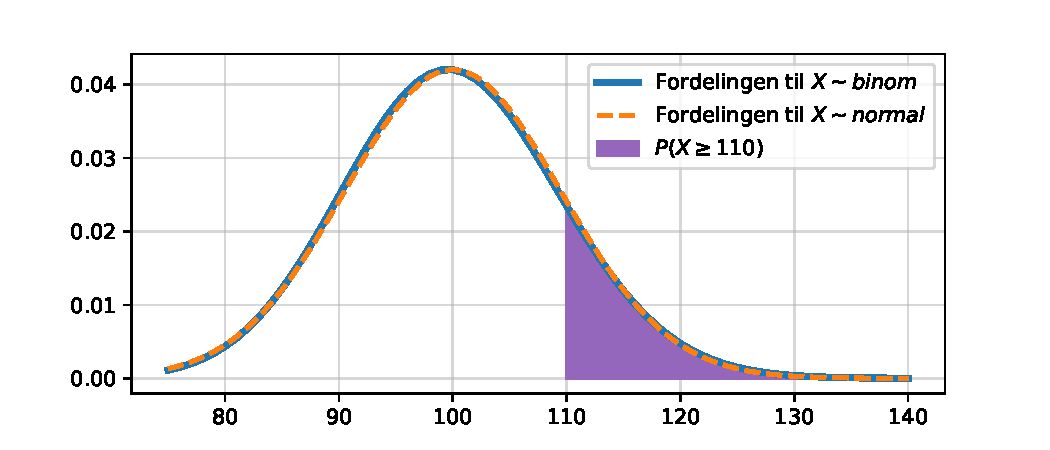
\includegraphics[width=0.85\linewidth]{figs/del2_oppg5}
\caption{Fordelingen til $X \sim \text{Binom}(n =1000, p=0.1)$, normalapproksimasjonen $X \sim \text{Normal}(\mu = np, \sigma^2 = np(1-p))$
	og arealet under grafen når $X\geq 110$.}
\label{fig:del2_oppg5}
\end{figure}

	# Vi setter opp hypotesene
	\begin{align*}
		H_0 &: \quad p = 0.1\\ 
		H_1 &: \quad p > 0.1\\ 
	\end{align*}
	og bruker signifikansnivå $5 \%$. 
	Vi forkaster nullhypotesen dersom sannsynligheten for å få
	$x_\text{obs}$ er  mindre enn $5 \%$, gitt at $p = 0.1$.
	I vårt tilfelle er $x_\text{obs} = 110$.
	Vi må finne sannsynligheten for at $X \geq x_\text{obs}$,
	gitt at $p = 0.1$.
	Med andre ord må vi finne $P(X \geq 110 \mid p = 0.1)$.
	
	## Det enkleste er å se på $X$ som binomisk fordelt med
	$n = 1000$ og $p = 0.1$, da gir sannsynlighetskalkulatoren
	i Geogebra oss at $P(X \geq 110) = 0.1583 = 15.5 \%$.
	Vi kan med andre ord \answer{ikke forkaste $H_0$}.
	
	## Her er også både $np$ og $n(p-1)$ større enn 5, så vi kan alternativt bruke
	normalapproksimasjon med $\mu =np=100 $ og $\sigma = \sqrt{1000 (0.1) (0.9)} = \sqrt{90}$. Normalapproksimasjonen er plottet i Figur \ref{fig:del2_oppg5}, og som du ser stemmer den veldig godt overens
	med den binomiske fordelingen.
	På eksamen ville jeg svart med binomisk fordeling, men jeg viser normalapproksimasjonen her.
	
	Vi regner ut $P(X \geq 110) \cong P(X_\text{norm} \geq 109.5) = 0.1583 = 15.5 \%$ i Geogebra. Legg merke til ``halvkorreksjon'', som brukes når vi går fra en diskret fordeling med søyler til en glatt, kontinuerlig fordeling. De første 4 desimalene er helt like, og konklusjonen er selvsagt den samme---vi forkaster $H_0$.
	
\end{easylist}

\subsection*{Oppgave 6}
\begin{easylist}[enumerate]
	\ListProperties(Style2*=,Numbers=a,Numbers1=l,FinalMark={)})
	# Vi beregner nåverdi for begge alternativene og setter de lik hverandre.
	
	\begin{center}
		\begin{tabular}{lll}
			Måned & Innbetaling & Nåverdi av innbetaling \\ \hline
			1 & $x$ & $\frac{x}{1.016}$ \\
			2 & $x$ & $\frac{x}{1.016^2}$ \\
			3 & $x$ & $\frac{x}{1.016^3}$ \\
			$\vdots$ & $\vdots$ \\
			36 & $x$ & $\frac{x}{1.016^{36}}$ \\
		\end{tabular}
	\end{center}
	Vi setter nåverdiene av innbetalingene lik dagens betaling, for får likning som vist i oppgaven.
	\begin{equation*}
		7995 + 30 = \frac{x}{1.016} + \frac{x}{1.016^2} + \dots + \frac{x}{1.016^{36}}
	\end{equation*}
	For å løse likningen på papir kan vi gange begge sider med $1.016^{36}$
	og bruke summeformelen for en geometrisk rekke.
	På eksamen er det nok enklere å bruke CAS, skriv 
	\verb|NLøs({8025 = Sum(x/1.016^i, i, 1, 36)}, {x})|,
	da får du at $\answer{x = 294.98 \text{ kr}}$.

	# Dette er samme problem som i forrige oppgaven, men nå er terminbeløpet kjent og renten er ukjent. Vi må løse
	\begin{equation*}
		7995 = \frac{289}{r} + \frac{289}{r^2} + \dots + \frac{289}{r^{36}},
	\end{equation*}
	der $r$ er den månedlige renten. Vi bruker CAS i Geogebra også her, og taster inn 
	\verb|NLøs({7995 = Sum(289/r^i, i, 1, 36)}, {r})| og finner at $r = 1.015$, slik at \answer{den månedlige renten er 1.5 \%}.
	
	# Dette er også en geometrisk rekke. Vi setter opp en tabell,
	der $r$ er den ukjente, månedlige renten.
	Hver måned får man rente på den eksisterende verdien, og nye 650 kr 
	blir satt inn. Dersom $V_n$ er verdien i år $n$, er $V_n = V_{n-1} r + 650$.
	
	\begin{center}
		\begin{tabular}{ll}
			Innbetaling & Verdi\\ \hline
			1 &  $650 $ \\
			2 &  $650 r + 650 $ \\
			3 &  $(650 r + 650)r + 650 = 650r^2 + 650r + 650 $ \\
			$\vdots$ & $\vdots$ \\
			12 & $650r^{11} + 650r^{10} + \dots + 650r^{2} + 650r + 650$ \\
		\end{tabular}
	\end{center}
	Like etter den 12. månedlige innbetalingen har hun 8107 kr,
	da får vi likningen 
	\begin{equation*}
		8107 = 650r^{11} + 650r^{10} + \dots + 650r^{2} + 650r + 650.
	\end{equation*}
	Det er også mulig å løse denne med summeformelen for en geometrisk rekke,
	men det er enklere å skrive \verb|NLøs({8107 = Sum(650*r^i, i, 0, 11)}, {r})| inn i CAS. Da finner vi ut at \answer{den månedlige renten er 0.7 \%}.
\end{easylist}

\subsection*{Oppgave 7}
Halveringstiden er 6 timer, men pasienten får én tablett hver 12. time.
Da rekker kroppen å halvere to ganger---med andre ord reduseres mengden med stoffet med $1/4$ hver 12. time.

\begin{center}
	\begin{tabular}{ll}
		Time & Milligram\\ \hline
		0 &  $60 $ \\
		12 &  $60/4 + 60$ \\
		24 &  $60/4^2 + 60/4 + 60$ \\
		36 &  $60/4^3 + 60/4^2 + 60/4 + 60$ \\
		$\vdots$ & $\vdots$
	\end{tabular}
\end{center}
Vi bruker formelen $1 + k + k^2 + \dots = 1 /(1 - k)$ til å regne ut summen $S$ av den evige geometriske rekken slik:
\begin{align*} 
	S &= 60 + \frac{60}{4}  + \frac{60}{4^2}  + \frac{60}{4^3} + \dots \\
	&= 60 \left( 1 +\frac{1}{4} + \frac{1}{4^2} + \frac{1}{4^3} + \dots  \right) \\
	&= 60 \left(  \frac{1}{1 - \frac{1}{4}}\right) = 60 \left(  \frac{1}{ \frac{3}{4}}\right)= 60 \left(  \frac{4}{ 3}\right)  = \answer{80}\\
\end{align*}
Du kan også skrive
\verb|Sum(60/4^i, i, 0, | $\infty$ \verb|)| inn i CAS. Du får samme svar.
På eksamen er det lurt å gjøre så mye som mulig i Geogebra,
men jeg prøver å vise at det er mulig å løse uten Geogebra også.


\end{document}


